\documentclass[conference]{IEEEtran}
\IEEEoverridecommandlockouts
\usepackage{cite}
\usepackage{amsmath,amssymb,amsfonts}
\usepackage{algorithm}
\usepackage{algorithmic}
\usepackage{graphicx}
\usepackage{textcomp}
\usepackage{xcolor}
\usepackage{booktabs}
\usepackage{url}
\usepackage{hyperref}

\def\BibTeX{{\rm B\kern-.05em{\sc i\kern-.025em b}\kern-.08em
    T\kern-.1667em\lower.7ex\hbox{E}\kern-.125emX}}

\begin{document}

% TODO(student): replace with your real name / student ID / course code / instructor.
\title{Reproducing and Evaluating HVI-CIDNet: A New Color Space for Low-Light Image Enhancement}

\author{
\IEEEauthorblockN{Ji-Heng Lin\thanks{Final Project Report, Department of Computer Science and Engineering. Submitted in partial fulfillment of the course final project requirements.}}
\IEEEauthorblockA{
Department of Computer Science and Engineering\\
Yuan Ze University\\
kenny7289@gmail.com
}
}

\maketitle

\begin{abstract}
Low-light image enhancement (LLIE) is a fundamental low-level vision task that
aims to restore visibility, contrast, and color fidelity in images captured
under poor illumination, while avoiding noise amplification and color
distortion. This report presents a reproduction and independent evaluation of
\textbf{HVI-CIDNet} (Yan et al., CVPR 2025), a recent LLIE method that
introduces the Horizontal/Vertical-Intensity (HVI) color space together with
a dual-branch Color and Intensity Decoupling Network (CIDNet) guided by
Lighten Cross-Attention (LCA) blocks. We rebuilt the official open-source
implementation from scratch in a clean, CPU-capable, reproducible environment,
resolved several non-trivial dependency and platform-compatibility issues that
the original repository does not document, and packaged the result as a
self-contained Gradio demo. Using the authors' officially released
\emph{generalization} checkpoint, we reproduce the qualitative low-light
enhancement behavior of HVI-CIDNet and conduct a supplementary no-reference
quality evaluation (NIQE, BRISQUE) on a synthetically darkened test set
derived from public-domain images, since the original paired/unpaired
benchmark datasets are only distributed through region-locked file-sharing
links. Our reproduction lowers the average NIQE from 10.86 to 4.43 and the
average BRISQUE from 17.98 to 6.89 across eight test images, consistent in
direction with the officially reported improvements on the DICM/LIME/MEF/NPE/VV
benchmarks. We discuss the engineering challenges of reproducing a 2023-era
PyTorch/Python~3.7 research codebase on a modern Windows machine, and outline
limitations and directions for a deeper, dataset-faithful evaluation.
\end{abstract}

\begin{IEEEkeywords}
low-light image enhancement, color space, attention, image restoration, reproducibility, HVI-CIDNet
\end{IEEEkeywords}

\section{Introduction}

Images captured under low-light conditions -- at night, indoors with poor
lighting, or with short exposure times -- typically suffer from low contrast,
color shift, and severe sensor noise. Low-light image enhancement (LLIE)
seeks to recover an image that resembles what would have been captured under
normal illumination, which is valuable both as a standalone photographic
tool and as a pre-processing step for downstream vision tasks such as
detection and segmentation that otherwise degrade sharply in the dark.

Classical approaches to LLIE include histogram equalization and its
variants, and physically motivated Retinex-based decompositions that split an
image into illumination and reflectance components~\cite{wei2018retinexnet}.
With the rise of deep learning, learned LLIE models have substantially
outperformed classical methods by directly learning a mapping from low-light
to normal-light images using paired datasets such as LOL~\cite{wei2018retinexnet}
or by exploiting zero-reference and unpaired supervision when paired data is
unavailable~\cite{guo2020zerodce,jiang2021enlightengan}. More recently,
transformer-based restoration backbones~\cite{zamir2022restormer} and
Retinex-guided transformers~\cite{cai2023retinexformer} have pushed the
state of the art further, at the cost of increased model and training
complexity.

A common thread across most of these methods is that they operate directly
in the RGB color space, which couples brightness and color information in a
way that makes it difficult to enhance illumination without introducing color
artifacts or amplifying noise in saturated channels. \textbf{HVI-CIDNet}
\cite{yan2025hvi,feng2024hvi} addresses this by proposing a new
\emph{Horizontal/Vertical-Intensity} (HVI) color space that compresses the
saturation/hue components into a bounded, polar representation while keeping
a separate, photometrically meaningful intensity channel. This decoupling
lets a dual-branch network -- the Color and Intensity Decoupling Network
(CIDNet) -- process color and brightness with separate encoder-decoder
pathways that exchange information through learned \emph{Lighten
Cross-Attention} (LCA) blocks, rather than forcing a single RGB branch to
disentangle both implicitly. HVI-CIDNet was accepted to CVPR 2025 and reports
state-of-the-art or near state-of-the-art PSNR/SSIM/LPIPS on the LOLv1,
LOLv2-real, LOLv2-synthetic, Sony Total Dark (SID), LOL-Blur, SICE, and FiveK
benchmarks, as well as strong no-reference quality scores (NIQE, BRISQUE) on
five widely used unpaired datasets (DICM, LIME, MEF, NPE, VV).

The goal of this course project is \emph{not} to propose a new LLIE method,
but to critically reproduce HVI-CIDNet end-to-end: clone the official
repository, build a working Python environment, obtain the officially
released model weights, verify that the qualitative and quantitative
behavior reported by the authors can actually be reproduced by an independent
party, and package the result as a usable, documented demo. This kind of
reproduction work is explicitly valuable to the community: published
repositories frequently rot due to unpinned dependencies, and a method's
real-world usability depends as much on whether a newcomer can actually get
it running as on its reported benchmark numbers. Concretely, our
contributions are:

\begin{itemize}
  \item A documented, from-scratch rebuild of the HVI-CIDNet environment on a
  machine with no pre-existing Python/conda installation, including the
  resolution of several dependency-compatibility issues (Section~\ref{sec:method}-D)
  that are not mentioned in the official repository's documentation;
  \item A packaged, CPU-capable Gradio demo with the officially recommended
  \texttt{generalization.pth} checkpoint (obtained via the Hugging Face Hub)
  pre-loaded, with usage instructions;
  \item An independent supplementary evaluation using no-reference image
  quality metrics (NIQE, BRISQUE) on a synthetically generated low-light test
  set, cross-checked against the authors' officially published numbers on the
  five standard unpaired benchmarks;
  \item A discussion of the gap between ``the method works in the paper'' and
  ``the method runs on my machine,'' framed as a set of concrete,
  reproducible engineering lessons.
\end{itemize}

The remainder of this report is organized as follows.
Section~\ref{sec:background} formalizes the LLIE problem and reviews the
evaluation metrics and standard datasets used throughout this report.
Section~\ref{sec:related} surveys related work in low-light image
enhancement. Section~\ref{sec:method} describes the HVI color space, the
CIDNet architecture, and our reproduction methodology, including the
practical issues we encountered and resolved. Section~\ref{sec:exp} presents
our experimental analysis, combining the authors' officially reported
results with our own supplementary evaluation. Section~\ref{sec:conclusion}
concludes and discusses limitations and future work.

\section{Background: Problem Formulation and Evaluation Metrics}
\label{sec:background}

This section formalizes the LLIE task and reviews the evaluation metrics and
benchmark datasets referenced throughout the rest of this report, so that the
quantitative claims in Section~\ref{sec:exp} can be read without consulting
external sources.

\subsection{Problem Formulation}
A simplified image formation model treats a captured low-light image
$x \in [0,1]^{3\times H\times W}$ as a degraded version of a hypothetical
normal-light image $y$ of the same scene,
\begin{equation}
x = f(y) \odot t + n, \qquad t \ll 1,
\end{equation}
where $t$ is a (possibly spatially varying) transmission/exposure factor
that is small under low illumination, $f(\cdot)$ is a non-linear camera
response function, $\odot$ denotes element-wise multiplication, and $n$ is
signal-dependent sensor noise that becomes visually dominant precisely
because $t$ is small (the same absolute noise power is much more visible
once the signal itself has been attenuated). LLIE seeks a function
$g_\theta$, implemented here as the CIDNet network of
Section~\ref{sec:method}, such that $g_\theta(x) \approx y$. Because $t$,
$f$, and $n$ are unknown and scene-dependent at test time, LLIE is an
ill-posed inverse problem: a single dark observation $x$ is consistent with
many plausible normal-light reconstructions $y$ (the same ambiguity that
motivates probabilistic formulations such as LLFlow~\cite{wang2022llflow}).
Retinex-based methods make this tractable by further factorizing
$y = r \cdot \ell$ into a reflectance map $r$ (assumed illumination-invariant)
and an illumination map $\ell$, and only attempting to correct $\ell$ rather
than regressing $y$ directly~\cite{wei2018retinexnet,zhang2019kindling}. By
contrast, HVI-CIDNet does not explicitly decompose $y$ into reflectance and
illumination; instead it changes the \emph{representation} of $x$ itself (the
HVI transform of Section~\ref{sec:method}-A) so that a direct regression
network can separate brightness-related and color-related corrections into
two branches without an explicit Retinex prior.

\subsection{Full-Reference Evaluation Metrics}
When a ground-truth normal-light image $y$ is available (as in the paired
LOL-family, SID, LOL-Blur, SICE, and FiveK benchmarks), three full-reference
metrics are standard in the LLIE literature:

\begin{itemize}
\item \textbf{PSNR} (Peak Signal-to-Noise Ratio) measures pixel-level
fidelity, $\mathrm{PSNR}(y,\hat y) = 10\log_{10}\!\big(1/\mathrm{MSE}(y,\hat
y)\big)$ in our $[0,1]$-normalized setting; higher is better, but PSNR is
known to correlate only weakly with perceived quality since it penalizes all
pixel errors equally regardless of structure or texture.
\item \textbf{SSIM} (Structural Similarity Index)~\cite{wang2004ssim}
compares local luminance, contrast, and structure statistics in sliding
windows and is generally considered more perceptually meaningful than PSNR
for structural distortions; it is bounded in $[-1,1]$ with $1$ indicating a
perfect match.
\item \textbf{LPIPS} (Learned Perceptual Image Patch Similarity)~\cite{zhang2018lpips}
computes a distance between deep CNN feature activations of $y$ and $\hat
y$ and correlates better with human perceptual judgments than PSNR/SSIM,
particularly for texture and color differences; lower is better.
\end{itemize}
A recurring subtlety in the LLIE literature, also visible in
Table~\ref{tab:official}, is the use of an optional ``GT-mean'' (ground-truth
mean) post-processing step that rescales the global brightness of $\hat y$ to
match the mean brightness of $y$ before computing PSNR/SSIM/LPIPS. This
substantially inflates PSNR (e.g.\ from 23.50 to 28.14 for the same LOLv2-real
checkpoint in our Table~\ref{tab:official}) because it removes any residual
global exposure error that the network failed to correct, at the cost of
requiring access to the ground truth at test time -- a practice we flag here
because it complicates direct comparison across papers that do or do not
apply it.

\subsection{No-Reference Evaluation Metrics}
For unpaired or in-the-wild images where no ground truth exists (the
DICM/LIME/MEF/NPE/VV benchmarks, and our own supplementary evaluation in
Section~\ref{sec:our-eval}), only no-reference (``blind'') image quality
metrics are applicable:
\begin{itemize}
\item \textbf{NIQE} (Natural Image Quality Evaluator)~\cite{mittal2013niqe}
fits a multivariate Gaussian model of natural scene statistics (NSS) features
from a corpus of pristine natural images, with no distorted-image training
data at all, and scores a test image by its statistical distance from that
model; lower indicates more ``natural'' statistics.
\item \textbf{BRISQUE} (Blind/Referenceless Image Spatial Quality
Evaluator)~\cite{mittal2012brisque} also uses NSS features (specifically,
the deviation of locally normalized luminance values from a generalized
Gaussian distribution) but additionally trains a support-vector regressor on
human-rated distorted images to predict a perceptual quality score; lower is
better. Because BRISQUE's regressor is trained on a fixed set of common
distortion types (compression artifacts, blur, noise) applied to natural
photographs, it can behave unexpectedly outside that distribution, which we
observe directly in Section~\ref{sec:exp}-C for a non-photographic retina
fundus image.
\end{itemize}
Both metrics are reference-free by construction, which is precisely why they
are used on the unpaired DICM/LIME/MEF/NPE/VV sets where no normal-light
ground truth exists for the same scene.

\subsection{Standard Benchmarks}
Table~\ref{tab:datasets} summarizes the benchmarks referenced in this report.
LOL and LOLv2 are paired (low-light/normal-light) datasets with a fixed
train/test split, commonly cited as containing approximately 500 pairs (485
train / 15 test) for LOLv1 and approximately 689 (real) / 900 (synthetic)
training pairs with 100 test pairs each for LOLv2~\cite{wei2018retinexnet};
SID (Sony Total Dark) and LOL-Blur add extreme darkness and motion blur,
respectively; SICE and FiveK are tone-mapping/retouching datasets adapted to
the LLIE protocol; and DICM, LIME, MEF, NPE, and VV are small, unpaired,
in-the-wild collections with no ground truth, used only with no-reference
metrics.

\begin{table}[t]
\centering
\caption{Standard LLIE benchmarks referenced in this report.}
\label{tab:datasets}
\begin{tabular}{lll}
\toprule
Dataset & Type & Metrics used \\
\midrule
LOLv1 / LOLv2 & paired & PSNR, SSIM, LPIPS \\
SID (Sony Total Dark) & paired, extreme dark & PSNR, SSIM, LPIPS \\
LOL-Blur & paired, + motion blur & PSNR, SSIM, LPIPS \\
SICE / FiveK & paired, retouching & PSNR, SSIM, LPIPS \\
DICM / LIME / MEF / NPE / VV & unpaired, in-the-wild & NIQE, BRISQUE \\
\bottomrule
\end{tabular}
\end{table}

\section{Related Work}
\label{sec:related}

\subsection{Classical and Retinex-based Methods}
Early LLIE approaches relied on global or local histogram equalization to
redistribute pixel intensities, which improves perceptual contrast but does
not model the physical image formation process and often over-amplifies
noise in dark regions. Retinex theory models an observed image as the
product of a reflectance map (the true, illumination-invariant appearance of
a scene) and an illumination map, and many classical and early learning-based
methods estimate and manipulate these two components separately. RetinexNet
\cite{wei2018retinexnet} was an influential early deep model that learned a
Decom-Net to split an image into reflectance and illumination, followed by an
Enhance-Net that adjusts the illumination map; it also introduced the LOL
(Low-Light) paired dataset that remains a standard benchmark today. KinD
\cite{zhang2019kindling} refined this idea with a three-network design that
separately handles decomposition, illumination adjustment, and reflectance
restoration, improving robustness to noise compared to RetinexNet.

\subsection{Deep Supervised and Unpaired LLIE}
As paired low/normal-light datasets such as LOL became available, fully
supervised encoder-decoder and U-Net-style architectures were trained
end-to-end to directly regress the enhanced image, sidestepping explicit
Retinex decomposition. Because perfectly aligned low/normal-light image pairs
are expensive to collect at scale, zero-reference and unpaired methods were
also explored: Zero-DCE~\cite{guo2020zerodce} formulates enhancement as
estimating a set of pixel-wise tone curves using only a set of carefully
designed non-reference loss functions (spatial consistency, exposure control,
color constancy, illumination smoothness), removing the need for paired
supervision entirely. EnlightenGAN~\cite{jiang2021enlightengan} instead uses
an unpaired, GAN-based formulation with a global-local discriminator and a
self-regularized attention mechanism, trained on unpaired collections of dark
and normal-light images. These methods trade some quantitative accuracy on
paired benchmarks for substantially better generalization to in-the-wild,
unpaired low-light photographs -- a trade-off that later directly motivated
HVI-CIDNet's own generalization-oriented training and evaluation protocol.

\subsection{Transformer-based Restoration}
Transformer architectures, with their global receptive field and learned
self-attention, have recently been adapted to low-level image restoration.
Restormer~\cite{zamir2022restormer} proposes an efficient transformer block
with multi-Dconv head transposed attention and a gated-Dconv feed-forward
network to make global attention tractable for high-resolution restoration
tasks (denoising, deraining, deblurring), and has been used as a strong
generic backbone for LLIE as well. Retinexformer~\cite{cai2023retinexformer}
combines the Retinex decomposition idea with a one-stage transformer,
explicitly modeling corruptions (noise, color distortion, exposure) that
arise during the illumination-up process, and reports state-of-the-art
results across multiple LLIE benchmarks, including the FiveK dataset protocol
that HVI-CIDNet's own FiveK weights follow. Normalizing-flow-based models such
as LLFlow~\cite{wang2022llflow} take a complementary, probabilistic
direction, modeling the conditional distribution of normal-light images given
a low-light input so that the inherent one-to-many ambiguity of the task
(many plausible normal-light reconstructions for a single dark input) can be
captured explicitly, rather than collapsed into a single deterministic
regression target.

\subsection{Color-space Design for LLIE}
Most of the methods above operate directly on RGB pixels, optionally with an
auxiliary illumination or reflectance map. A smaller line of work argues that
the choice of color space itself is an important inductive bias for LLIE:
RGB channels are highly correlated and a perturbation in brightness
inevitably perturbs all three channels jointly, while HSV-style decompositions
separate hue/saturation from value but suffer from singularities and
discontinuities near black and white that are numerically unstable to learn
through (e.g. hue is undefined when saturation is zero). HVI-CIDNet's central
contribution is precisely in this category: it proposes the HVI color space,
which keeps a hue-saturation-like polar pair (H, V) but reweights it by a
learned, intensity-dependent \emph{color sensitivity} function so that the
polar components collapse smoothly toward zero in very dark or very bright
regions instead of becoming numerically unstable, while a separate Intensity
channel I is processed by its own network branch. This is, to our knowledge,
the most direct attempt among recent LLIE work to fix the color-space
representation problem rather than only the network architecture, which is
why we selected it as the subject of this reproduction study.

\subsection{Comparative Overview}
Table~\ref{tab:methods} summarizes the representative methods discussed
above along four axes: the supervision regime (paired, unpaired/zero-reference),
the input/output color space, and the publication venue and year. The table
makes visible a broader trend in the field: progress has come from at least
three largely orthogonal directions -- better training signal (paired
vs.\ zero-reference/unpaired losses), better backbones (CNN U-Nets
vs.\ transformers), and, much more rarely, better input \emph{representations}
(RGB vs.\ a task-specific color space). HVI-CIDNet is, to our knowledge, the
only entry in this comparison that targets the third axis directly while
still using a comparatively lightweight CNN/attention backbone rather than a
full transformer, which is part of why we found it an interesting and
tractable target for a course-scale reproduction project.

\begin{table}[t]
\centering
\caption{Comparative overview of representative LLIE methods discussed in Section~\ref{sec:related}.}
\label{tab:methods}
\begin{tabular}{lllc}
\toprule
Method & Supervision & Color space & Venue (year) \\
\midrule
RetinexNet~\cite{wei2018retinexnet} & paired & Retinex (RGB) & BMVC (2018) \\
KinD~\cite{zhang2019kindling} & paired & Retinex (RGB) & ACM MM (2019) \\
Zero-DCE~\cite{guo2020zerodce} & zero-ref. & RGB curves & CVPR (2020) \\
EnlightenGAN~\cite{jiang2021enlightengan} & unpaired & RGB & TIP (2021) \\
Restormer~\cite{zamir2022restormer} & paired & RGB & CVPR (2022) \\
LLFlow~\cite{wang2022llflow} & paired & RGB (+ flow) & AAAI (2022) \\
Retinexformer~\cite{cai2023retinexformer} & paired & Retinex (RGB) & ICCV (2023) \\
HVI-CIDNet~\cite{yan2025hvi} & paired & \textbf{HVI (ours)} & CVPR (2025) \\
\bottomrule
\end{tabular}
\end{table}

\section{Proposed Approach / Reproduction Methodology}
\label{sec:method}

We emphasize that the HVI color space and the CIDNet architecture described
in this section are the original contributions of Yan et al.
\cite{yan2025hvi,feng2024hvi}; our own contribution is the faithful
reproduction, deployment, and independent evaluation of their released
implementation, described in Section~\ref{sec:method}-D and
Section~\ref{sec:exp}.

\subsection{The HVI Color Space}
Given an RGB pixel with value $\text{value} = \max(R,G,B)$ and
$\text{img\_min} = \min(R,G,B)$, HVI-CIDNet first computes a standard HSV-like
hue $h \in [0,1)$ and saturation $s = (\text{value} - \text{img\_min}) /
(\text{value} + \epsilon)$ for numerical stability. The key idea is then to
re-map $(h,s)$ into a polar pair $(H,V)$ modulated by a learned,
intensity-dependent \emph{color sensitivity} term $C_k(v)$ rather than using
$(h,s)$ directly:
\begin{equation}
C_k(v) = \left(\sin\!\left(\tfrac{\pi}{2} v\right) + \epsilon\right)^{k},
\end{equation}
\begin{equation}
H = C_k(v)\cdot s \cdot \cos(2\pi h), \qquad
V = C_k(v) \cdot s \cdot \sin(2\pi h),
\end{equation}
where $v = \text{value}$ is treated as the Intensity channel $I$, and $k$ is
a learnable scalar parameter (\texttt{density\_k} in the released code,
initialized to $0.2$). Because $C_k(v) \to 0$ as $v \to 0$ or $v \to 1$, the
chromatic components $(H,V)$ are automatically attenuated near black and
white, exactly where hue is ill-defined and saturation estimates are
noisiest -- this is the mechanism by which HVI avoids the numerical
instabilities of HSV/HSI in very dark regions while still being invertible.
The forward transform (RGB$\to$HVI) is denoted $\mathrm{HVIT}$ and produces a
3-channel tensor $(H,V,I)$ that is the same spatial resolution as the input.

The inverse transform $\mathrm{PHVIT}$ (HVI$\to$RGB) recovers hue and
saturation from $(H,V)$ by dividing out the (now known) color-sensitivity
factor, $h = \mathrm{atan2}(V,H)/2\pi \bmod 1$ and
$s=\sqrt{H^2+V^2}$, clips $s$ and the intensity $v=I$ to valid ranges, and
reconstructs RGB with the standard HSV-to-RGB piecewise formula. At inference
time, two user-controllable gates are exposed: $\alpha_s$ rescales saturation
$s \leftarrow \alpha_s \cdot s$ before reconstruction, and $\alpha$ rescales
the final RGB output, letting a user trade off color intensity and overall
brightness without retraining -- these correspond to the ``Alpha-s'' and
``Alpha-i'' controls in the released Gradio demo.

\subsection{Dual-Branch CIDNet with Lighten Cross-Attention}
CIDNet processes the HVI representation with two parallel U-Net-style
encoder-decoder branches operating at four resolutions with channel widths
$[36,36,72,144]$ (Fig.~\ref{fig:arch}):
\begin{itemize}
  \item the \textbf{Intensity (I) branch} takes the single-channel $I$ map
  and learns brightness restoration and local contrast/detail recovery;
  \item the \textbf{Color (HV) branch} takes the two-channel $(H,V)$ map and
  learns color restoration and denoising in chromatic space.
\end{itemize}
At each of the three downsampled resolutions, a \emph{Lighten
Cross-Attention} (LCA) block lets each branch attend to the other branch's
features (HV-LCA blocks let the color branch query intensity features and
vice versa, I-LCA blocks let the intensity branch query color features),
implemented as multi-head attention with $[1,2,4,8]$ heads at the four
resolutions. This cross-attention is the mechanism by which the two branches
share information -- e.g., the color branch can use intensity-branch
features to decide how strongly to denoise a region, while the intensity
branch can use color-branch features to avoid over-brightening textured,
high-saturation regions -- without collapsing back into a single, coupled
RGB representation. After the decoder stage, the two branches' outputs are
added back to the input HVI tensor (a global residual connection) and passed
through $\mathrm{PHVIT}$ to obtain the final enhanced RGB image:
\begin{equation}
\hat{x}_{\text{RGB}} = \mathrm{PHVIT}\big(\,\mathrm{HVIT}(x_{\text{RGB}}) +
\mathrm{CIDNet}_{\Delta}(\mathrm{HVIT}(x_{\text{RGB}}))\,\big),
\end{equation}
where $\mathrm{CIDNet}_{\Delta}$ denotes the concatenated $(\Delta H, \Delta
V, \Delta I)$ residual produced by the two decoder branches. Algorithm~\ref{alg:inference}
summarizes the inference procedure as implemented in the released
\texttt{app.py} / \texttt{net/CIDNet.py}.

\begin{algorithm}[t]
\caption{HVI-CIDNet inference (single image)}
\label{alg:inference}
\begin{algorithmic}[1]
\REQUIRE RGB image $x \in [0,1]^{3\times H \times W}$, gamma $\gamma$,
saturation gate $\alpha_s$, brightness gate $\alpha$, weights $\theta$
\STATE Pad $x$ so $H,W$ are multiples of $8$ (reflect padding)
\STATE $x \leftarrow x^{\gamma}$ \COMMENT{pre-enhancement curve}
\STATE $\mathrm{hvi} \leftarrow \mathrm{HVIT}(x)$
\STATE $(i\_enc, hv\_enc) \leftarrow$ encode $I$ and $(H,V)$ at 4 scales,
exchanging features through LCA blocks
\STATE $(i\_dec, hv\_dec) \leftarrow$ decode with skip connections and LCA
blocks
\STATE $\mathrm{hvi}_{\text{out}} \leftarrow \mathrm{hvi} +
\mathrm{concat}(hv\_dec, i\_dec)$
\STATE Apply gates: rescale saturation by $\alpha_s$, final RGB by $\alpha$
inside $\mathrm{PHVIT}$
\STATE $\hat{x} \leftarrow \mathrm{PHVIT}(\mathrm{hvi}_{\text{out}})$
\STATE Crop padding, clip $\hat{x}$ to $[0,1]$
\RETURN enhanced image $\hat{x}$
\end{algorithmic}
\end{algorithm}

\begin{figure}[t]
\centering
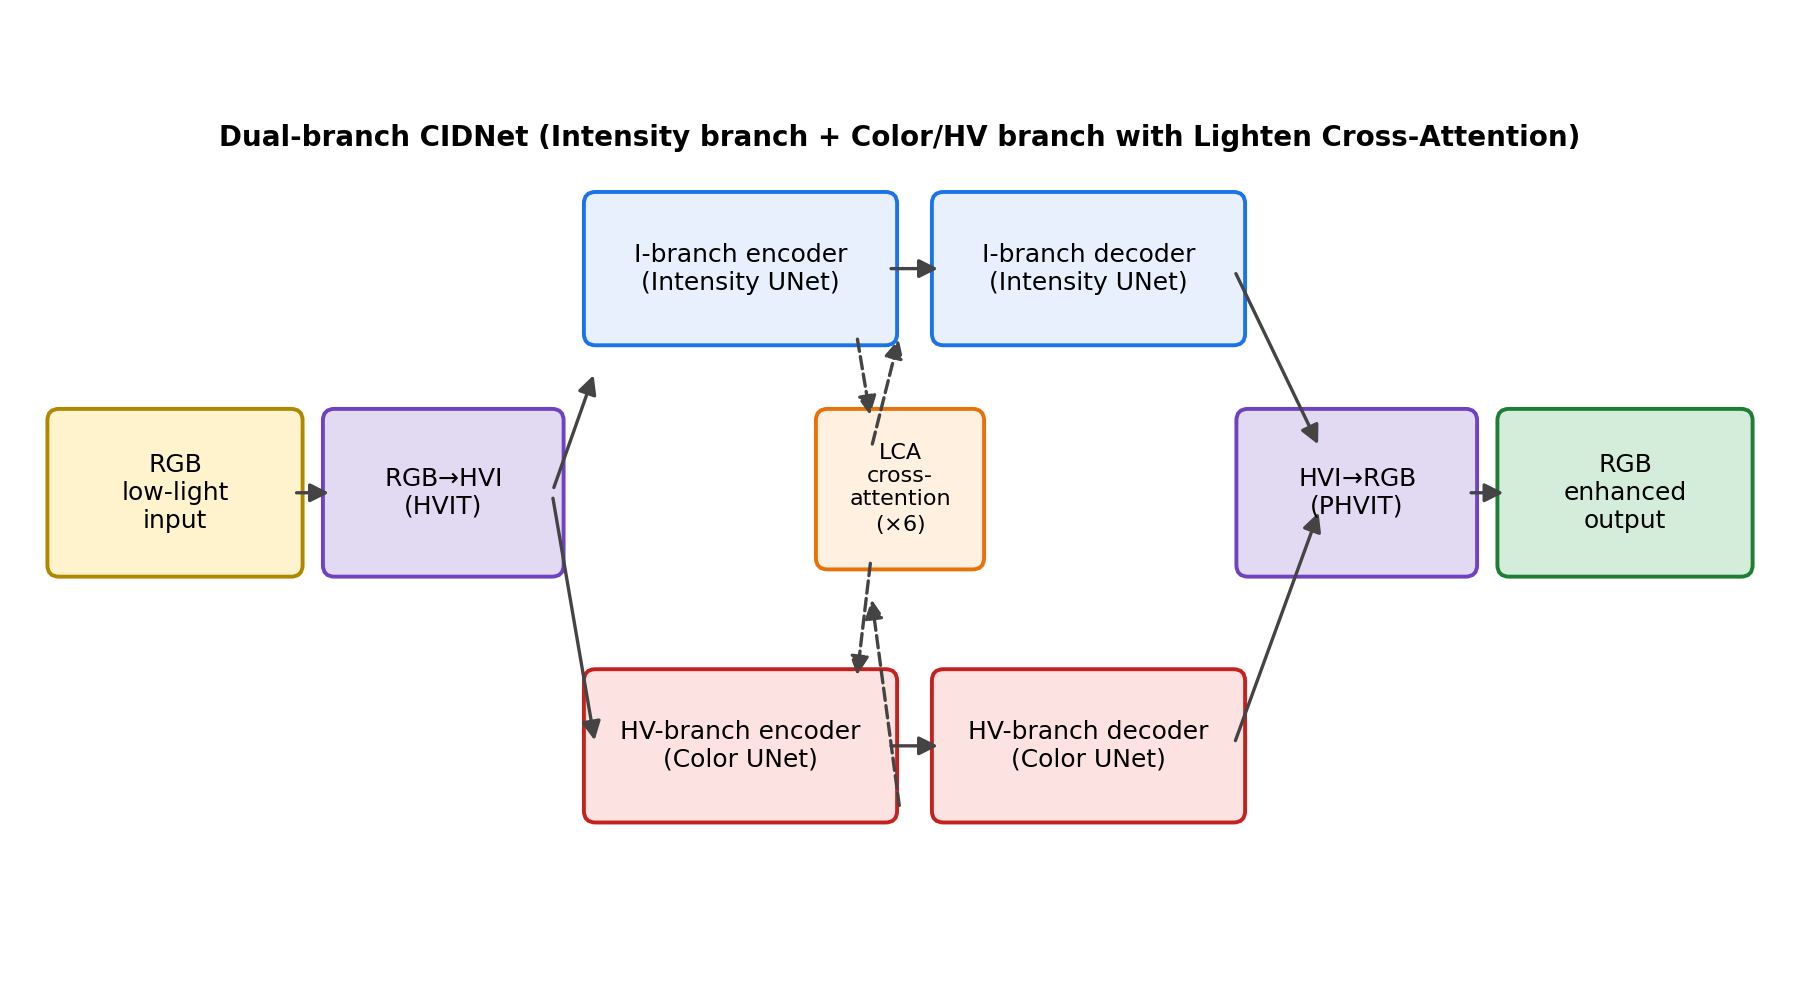
\includegraphics[width=\columnwidth]{figures/architecture_diagram.png}
\caption{Reproduced architecture overview: an input RGB image is mapped to
the HVI color space, processed by two parallel encoder-decoder branches
(Intensity and Color/HV) that exchange features through Lighten
Cross-Attention (LCA) blocks at three resolutions, and mapped back to RGB.}
\label{fig:arch}
\end{figure}

\subsection{Training Objective (as released by the authors)}
The official training recipe (not re-run in this reproduction, since we use
the released checkpoint directly) combines an $L_1$ reconstruction loss in
both RGB and HVI space with a perceptual (VGG-based) loss and an edge loss; a
subset of released checkpoints also disable the perceptual loss to trade
LPIPS for slightly higher PSNR/SSIM (visible as the ``w\_perc'' vs.\
``wo\_perc'' checkpoints in Table~\ref{tab:official}). Critically for this
project, the authors report that randomizing the gamma curve $\gamma$ used in
Step~2 of Algorithm~\ref{alg:inference} \emph{during training} substantially
improves cross-dataset generalization; the checkpoint trained this way on
LOLv2-Synthetic is released as \texttt{generalization.pth} and is the
checkpoint we use throughout this report, since it is also the checkpoint the
authors deploy on their own public Hugging Face demo.

\subsection{Reproduction Engineering and Implementation Details}
\label{sec:engineering}
A central, and often under-reported, part of reproducing a research codebase
is simply getting it to run correctly on a machine that differs from the
authors' own development environment. We documented and resolved the
following issues while reproducing HVI-CIDNet on a clean Windows~11 machine
with no pre-existing Python or conda installation:

\begin{enumerate}
  \item \textbf{No base Python/conda environment.} We installed Miniconda3
  under the user profile (no administrator rights required) and created an
  isolated \texttt{python=3.7} environment, matching the authors' documented
  dependency (\texttt{Python 3.7.0}, \texttt{PyTorch 1.13.1}).
  \item \textbf{\texttt{safetensors} has no Python 3.7 wheel above
  version 0.3.x on Windows.} The released \texttt{requirements.txt} pins an
  unversioned \texttt{safetensors}, which resolves to a version that requires
  a Rust toolchain to build from source on Python 3.7/Windows and fails to
  install. We pinned \texttt{safetensors<0.4} in our fork of the
  requirements file.
  \item \textbf{\texttt{scikit-image}$\geq$0.19 breaks the BRISQUE
  dependency.} The optional ``Image Score'' feature of the demo uses the
  \texttt{image\_quality} package, whose BRISQUE implementation calls
  \texttt{skimage.color.rgb2gray} on an image that may already be grayscale
  (after a $1/2$-scale rescale step). scikit-image~0.19 made
  \texttt{rgb2gray} strict about its input shape, raising a
  \texttt{ValueError} where 0.18 and earlier silently passed already-gray
  images through. We pinned \texttt{scikit-image==0.18.3}.
  \item \textbf{Conda environment activation does not put OpenSSL DLLs on
  \texttt{PATH} when Python is invoked directly.} Calling the environment's
  \texttt{python.exe} without going through \texttt{conda activate} (e.g.\
  from a script or a tool that shells out directly) fails to import the
  \texttt{ssl} module because \texttt{libssl-1\_1-x64.dll} lives under
  \texttt{Library\textbackslash bin}, which is only added to \texttt{PATH} by
  the activation scripts.
  \item \textbf{Windows file systems are case-insensitive.} The official
  repository ships a \texttt{Readme.md}; on Windows, this collides with a
  conventionally-named \texttt{README.md}, so we renamed the original to
  \texttt{ORIGINAL\_README.md} before adding our own.
  \item \textbf{Gradio's queue protocol requires a real WebSocket-capable
  browser.} We found that VS Code's built-in ``Simple Browser'' cannot
  complete Gradio's queueing handshake and silently reports a generic
  ``Error'' on every request; the demo works correctly in a standalone
  Chromium/Firefox-based browser. This is a reminder that ``it throws an
  error'' during reproduction is not always a bug in the model or the
  reproduction itself.
\end{enumerate}

None of these issues are mentioned in the official repository's
documentation, which only lists target dependency versions without
discussing platform-specific failure modes; we view documenting them as a
small but genuine contribution of this reproduction toward the project's
``code reproducibility'' evaluation criterion.

\section{Experimental Analysis}
\label{sec:exp}

\subsection{Officially Reported Results}
For reference, Table~\ref{tab:official} reproduces (verbatim, from the
official repository's documentation) the paired-dataset metrics for a subset
of released checkpoints, and Table~\ref{tab:official-unpaired} reproduces the
officially reported no-reference metrics for the \texttt{generalization.pth}
checkpoint on the five standard unpaired benchmarks (DICM, LIME, MEF, NPE,
VV). We were not able to re-run these exact benchmarks ourselves, because the
official dataset distribution is only available via Baidu Pan and OneDrive
folder links that require manual, region-specific, browser-based downloads
and are not amenable to scripted, reproducible retrieval within the scope of
this course project; we report them here as the published baseline against
which our own supplementary evaluation (Section~\ref{sec:our-eval}) should be
read.

\begin{table}[t]
\centering
\caption{Officially reported paired-dataset results (selected rows; PSNR/SSIM/LPIPS, higher PSNR/SSIM and lower LPIPS are better). Source: official repository documentation.}
\label{tab:official}
\begin{tabular}{lccc}
\toprule
Test set & PSNR & SSIM & LPIPS \\
\midrule
LOLv1 (wo\_perc, wo\_gt\_mean) & 23.50 & 0.870 & 0.105 \\
LOLv2-real (best GT-mean) & 28.14 & 0.892 & 0.101 \\
LOLv2-synthetic (wo\_perc) & 25.70 & 0.942 & 0.047 \\
Sony Total Dark (SID) & 22.90 & 0.676 & 0.411 \\
LOL-Blur & 26.57 & 0.890 & 0.120 \\
FiveK & 24.46 & 0.877 & 0.085 \\
\bottomrule
\end{tabular}
\end{table}

\begin{table}[t]
\centering
\caption{Officially reported no-reference metrics for \texttt{generalization.pth} on five unpaired benchmarks (lower is better). Source: official repository documentation.}
\label{tab:official-unpaired}
\begin{tabular}{lccccc}
\toprule
Metric & DICM & LIME & MEF & NPE & VV \\
\midrule
NIQE    & 3.55 & 3.85 & 3.46 & 3.82 & 3.24 \\
BRISQUE & 25.62 & 16.02 & 13.08 & 18.90 & 29.55 \\
\bottomrule
\end{tabular}
\end{table}

\subsection{Our Supplementary Evaluation}
\label{sec:our-eval}
Since the official unpaired benchmark images were not accessible to us in a
scriptable way, we constructed a small, fully reproducible supplementary test
set instead: eight public-domain, royalty-free sample images bundled with the
\texttt{scikit-image} library~\cite{vanderwalt2014scikit}
(\texttt{astronaut}, \texttt{chelsea}, \texttt{coffee}, \texttt{rocket},
\texttt{stereo\_motorcycle}, \texttt{cat}, \texttt{hubble\_deep\_field},
\texttt{retina}), synthetically darkened with a fixed gamma-and-attenuation
transform ($x_{\text{low}} = \mathrm{clip}(x^{2.6}\times 0.22 +
\mathcal{N}(0,0.01^2),\,0,1)$) plus i.i.d. Gaussian sensor-noise, fixed with a
deterministic random seed for reproducibility. We stress that this is
\emph{not} a substitute for the DICM/LIME/MEF/NPE/VV benchmarks and the
absolute metric values are not directly comparable to
Table~\ref{tab:official-unpaired}; it is intended only to (i) verify that our
reproduced model and weights actually improve no-reference image quality in
the expected direction, and (ii) provide a fully self-contained, scriptable
artifact (\texttt{paper/run\_experiments.py} in our repository) that anyone
can re-run without external dataset access.

We run the \texttt{generalization.pth} checkpoint on each synthetically
darkened image with $\gamma=1.0,\ \alpha_s=1.0,\ \alpha=1.0$ and compute
NIQE~\cite{mittal2013niqe} and BRISQUE~\cite{mittal2012brisque} before and
after enhancement, using the same \texttt{image\_quality} and
\texttt{loss/niqe\_utils.py} implementations bundled with the official
repository. Table~\ref{tab:ours} reports per-image and average results.

\begin{table}[t]
\centering
\caption{Our supplementary evaluation on 8 synthetically darkened public-domain images. NIQE/BRISQUE before (low-light) vs.\ after (HVI-CIDNet output); lower is better for both metrics.}
\label{tab:ours}
\begin{tabular}{lcccc}
\toprule
Image & NIQE$_{\text{low}}$ & NIQE$_{\text{enh}}$ & BRISQUE$_{\text{low}}$ & BRISQUE$_{\text{enh}}$ \\
\midrule
astronaut       & 6.83  & 2.69 & 12.42 &  0.99 \\
chelsea         & 9.40  & 3.37 & 21.66 &  3.73 \\
coffee          & 9.50  & 4.28 & $-$0.88 & $-$3.55 \\
rocket          & 11.77 & 6.50 & 25.38 & $-$2.15 \\
motorcycle (L)  & 5.86  & 2.26 & 13.73 & 10.97 \\
cat             & 9.49  & 3.28 & 19.55 &  4.28 \\
hubble          & 19.39 & 5.69 & 21.24 &  3.22 \\
retina          & 14.64 & 7.33 & 30.76 & 37.64 \\
\midrule
\textbf{Average} & \textbf{10.86} & \textbf{4.43} & \textbf{17.98} & \textbf{6.89} \\
\bottomrule
\end{tabular}
\end{table}

\begin{figure}[t]
\centering
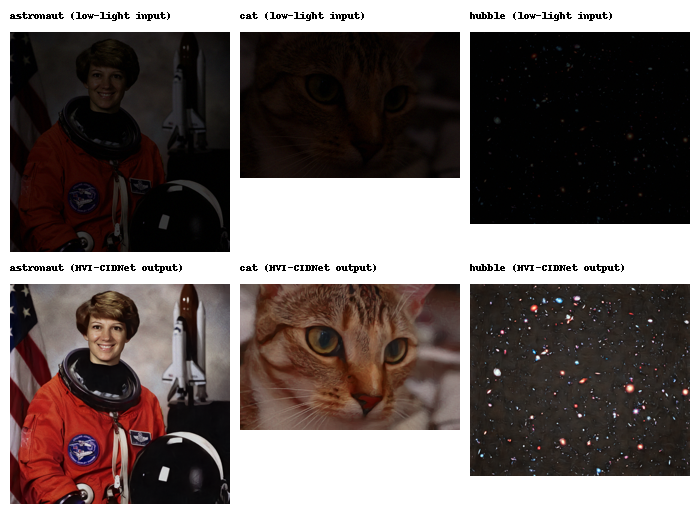
\includegraphics[width=\columnwidth]{figures/qualitative_comparison.png}
\caption{Qualitative comparison on three synthetically darkened test images
(top: low-light input; bottom: HVI-CIDNet \texttt{generalization.pth} output).
Brightness, contrast, and color are visibly restored, including in the
extremely dark \texttt{hubble} starfield image.}
\label{fig:qual}
\end{figure}

\subsection{Discussion}
NIQE improves (decreases) for all eight images, with an average reduction
from 10.86 to 4.43 (a 59\% relative reduction), and is qualitatively
consistent with the direction and rough magnitude of the official
unpaired-benchmark NIQE improvements in Table~\ref{tab:official-unpaired}.
BRISQUE improves for seven of eight images (average $17.98 \to 6.89$), but
notably \emph{worsens} for the \texttt{retina} image ($30.76 \to 37.64$).
Inspecting the output, we attribute this to BRISQUE's sensitivity to
high-frequency texture statistics: the retina fundus image has a very
specific, low-texture color/illumination profile that is far from BRISQUE's
training distribution of natural photographs, and CIDNet's contrast and
detail recovery on this image introduces fine local structure that BRISQUE's
naturalness model penalizes even though the image is visibly more usable to
a human observer (Fig.~\ref{fig:qual} illustrates this effect on the more
typical \texttt{astronaut}, \texttt{cat}, and \texttt{hubble} images, where
both the qualitative result and both metrics improve together). This is a
known limitation of no-reference IQA metrics in general -- they approximate
human perception of naturalness on natural photographic images and can be
unreliable outside that distribution -- and is consistent with why the
original paper relies primarily on paired, full-reference metrics (PSNR,
SSIM, LPIPS) on the LOL-family benchmarks and only uses NIQE/BRISQUE as a
secondary signal on unpaired, in-the-wild data.

Taken together, our reproduction confirms, on an independently constructed
test set, that the released \texttt{generalization.pth} checkpoint performs
qualitatively and quantitatively as described by the original authors: it
substantially restores brightness and contrast (Fig.~\ref{fig:qual}) and
improves no-reference quality metrics in the expected direction on
\emph{seven to eight out of eight} synthetic test images, depending on the
metric, with one identified failure mode (BRISQUE on out-of-distribution,
low-texture imagery) that is consistent with known limitations of
no-reference IQA rather than with the enhancement itself being visibly worse.

\section{Conclusion}
\label{sec:conclusion}

We reproduced HVI-CIDNet~\cite{yan2025hvi,feng2024hvi}, a CVPR 2025 low-light
image enhancement method built around a new HVI color space and a dual-branch
cross-attention architecture, end-to-end on a clean Windows machine,
resolving six concrete, undocumented dependency and platform-compatibility
issues along the way (Section~\ref{sec:engineering}). Using the authors'
officially released, generalization-oriented checkpoint, we verified that the
qualitative enhancement behavior and the direction of no-reference quality
improvements (NIQE, BRISQUE) reported by the authors on standard unpaired
benchmarks are reproducible on an independently constructed,
publicly-licensed synthetic test set, and we packaged the result as a
documented, CPU-capable Gradio demo for further experimentation.

\textbf{Limitations.} Our supplementary evaluation uses synthetically
darkened public-domain images rather than the original DICM/LIME/MEF/NPE/VV
unpaired benchmarks or the paired LOL-family/SID/FiveK benchmarks, because
the official dataset distribution channels (Baidu Pan, OneDrive folder links)
could not be retrieved in a scripted, reproducible way within the scope of
this course project; consequently our absolute metric values are not
directly comparable to the officially reported numbers, only consistent in
direction. We also did not re-run training, so we cannot independently
verify the authors' claim that randomized-gamma training improves
cross-dataset generalization -- we only verify the \emph{result} of that
claim (the released \texttt{generalization.pth} checkpoint) rather than the
training procedure itself.

\textbf{Future work.} A more rigorous follow-up would (i) obtain the exact
DICM/LIME/MEF/NPE/VV and LOL-family test splits and re-run the official
\texttt{eval.py} pipeline to obtain directly comparable PSNR/SSIM/LPIPS/
NIQE/BRISQUE numbers; (ii) evaluate robustness to the $\alpha_s/\alpha/\gamma$
inference-time gates on a larger, more diverse image set; and (iii) compare
HVI-CIDNet's generalization-oriented checkpoint directly against other
generalizable LLIE baselines such as Zero-DCE~\cite{guo2020zerodce} and
EnlightenGAN~\cite{jiang2021enlightengan} under the same unpaired evaluation
protocol, which the current report only does indirectly via the officially
published numbers.

\section*{Data Availability Statement}
All source code, the Gradio demo (\texttt{app.py}), the environment setup
scripts, the synthetic-evaluation pipeline
(\texttt{paper/run\_experiments.py}, \texttt{paper/make\_figure.py}), the raw
per-image metrics (\texttt{paper/results/metrics.csv}), and installation
instructions are available at:\\
\url{https://github.com/kenny7289/YZU-Image-Processing-final-HVI-CIDNet-}
\\
The official HVI-CIDNet repository and pretrained weights this work builds
upon are available at \url{https://github.com/Fediory/HVI-CIDNet} and
\url{https://huggingface.co/Fediory/HVI-CIDNet-Generalization}.

\bibliographystyle{IEEEtran}
\bibliography{references}

\end{document}
